

\begin{frame}
\frametitle{Quantum theory of radiation by nonstationary systems 
	with application to high-order harmonic generation
        (Phys. Rev. A 101, 013410 (2020))}
        \framesubtitle{Part 2 - Solving $\boldsymbol{\phi_\omega(x,t)}$}
\footnotesize
\begin{textblock*}{400pt}(30pt,60pt)
\begin{itemize}
\item We are now interested in solving 
the following 1D problem with a ZRP
\begin{align}
\begin{cases}
	i\frac{\partial}{\partial t}\psi(x,t)
	   & = \left( \hat{H}_a + \hat{V}_{\rm ext}(t)\right) 
	   \psi(x,t),\\
	i\frac{\partial}{\partial t}\phi_\omega(x,t)
	   & = \left( \hat{H}_a + \hat{V}_{\rm ext}(t)\right) 
	   \phi_\omega (x,t)
%	   + e^{i\omega t} {\hat{p}}\,
%	   \psi(x,t), \label{eqn:main_1d} 
	   + e^{i\omega t} S(x,t)\,
\end{cases}
\end{align}
%\begin{equation}
%	i\frac{\partial}{\partial t}\phi_\omega(x,t)
%	   = \left( \hat{H}_a + \hat{V}_{\rm ext}(t)\right) 
%	   \phi_\omega (x,t)
% 	   + \alpha A_\omega e^{i\omega t} {\hat{p}}\,
%	   \psi(x,t), \label{eqn:main_1d}
%\end{equation}

where

\begin{equation}
  \hat{H}_a = -\frac{1}{2}\frac{d^2}{dx^2} - \varkappa\delta(x), 
	\hspace{20pt}  \hat{V}_{\rm ext}(t) = F(t)x, \hspace{20pt}
	S(x,t) = \hat{p}\,\psi(x,t)
\end{equation}
\begin{align}
  \phi_\omega (x,0) = \frac{-i\varkappa^{3/2}}{\omega}
	{\rm sgn}(x)\left(e^{-\varkappa|x|} - e^{-\varkappa(\omega)|x|}\right), &
\hspace{20pt}  \psi(x,0) = \varkappa^{1/2}e^{-\varkappa|x|}, 
\label{eqn:bound_state0} \\
	\hat{p} = -id/dx,\hspace{10pt}  \mbox{ and } 
	\hspace{10pt} \varkappa(\omega) & = \sqrt{\varkappa^2 + 2\omega}.
\end{align}
%\begin{equation}
%  E_k = k^2/2,\hspace{20pt}
%  \psi_k^{(\pm)}(x) = e^{ikx} + R(\pm|k|)e^{\pm i|kx|}, \hspace{20pt}
%   R(k) = \frac{i\varkappa}{k-i \varkappa}. \label{eqn:inout_states}
%\end{equation}
%\item The parameters of the laser we will be using 
%are given by the relations
%\begin{equation}
%  F(t) = F_0 e^{-(2t^\prime/\tau)^2}\cos(\omega_0 t^\prime),\hspace{20pt}
%  0 \leqslant t^\prime \leqslant \tau
%\end{equation}
%\begin{equation}
%  \tau  = 2\pi n_{oc}/\omega,  \hspace{20pt}
%  F_0 = .1\,{\rm a.u.}, \hspace{20pt}
%  n_{oc} = 5, \hspace{20pt}
%  \omega_0 = 0.114\,{\rm a.u.}
%\end{equation}

%       \begin{equation}
%               \phi^\omega_{n+1} = U_4(\Delta t) \phi^\omega_{n}
%               - \frac{i\Delta t}{6}\left(
%                 U_4(\Delta t)  e^{i\omega t_{n}}     S_{n}
%               + 4 U_4(\Delta t/2) e^{i\omega t_{n+\frac{1}{2}}} S_{n+\frac{1}{2}}
%               +   U_4(0) e^{i\omega t_{n+1}} S_{n+1}
%               \right)
%                \label{eqn:simpson_duhamel}
%       \end{equation}
\begin{align}
        \phi_\omega(x,t) & = U(t,t_0)\phi_\omega(x,t_0)
          -i\int_{t_0}^tU(t-\tau)e^{i\omega \tau}S(x,\tau)d\tau. \label{eqn:duhamel}
\end{align}



\end{itemize}


%\begin{align}
%\psi(x,t)
% & = e^{-i(\mathcal{L}+ \hat{V}_{\rm ext})}\psi(x,0)    \nonumber\\
%\phi_\omega(x,t)
% & = e^{-i(\mathcal{L} + \hat{V}_{\rm ext})t}
%   \phi_\omega(x,0) 
%  - e^{-i(\mathcal{L} + \hat{V}_{\rm ext})t}
%   \int_0^t e^{i\omega s}\,\frac{\partial}{\partial x}\,\psi(x,s) e^{i(\mathcal{L} 
% + \mathcal{N})s}ds  \nonumber\\
% & = e^{-i(\mathcal{L} + \hat{V}_{\rm ext})t}
%  \left( \phi_\omega(x,0) 
%   -\int_0^t e^{i\omega s}\,\frac{\partial}{\partial x}\,\psi(x,s) 
%  e^{-i(\mathcal{L}+ \hat{V}_{\rm ext})s} ds\right)  \nonumber
%\end{align}                                                            %

\end{textblock*}

\begin{textblock*}{250pt}(240pt,80pt)
%\includegraphics[scale=.25]{dip_app_limits.png}{\footnote{\Tiny
%H.R. Reiss, Phys Rev A 63 013409 (2000)}}
\end{textblock*}

\end{frame}






\section{Propagation schemes}


\begin{frame}
\frametitle{High-order exponential splitting (composition methods)
        (Phys. Rev. A 101, 013410 (2020))}
%\frametitle{Geometric propagators}
	\framesubtitle{Yoshida (1990) - 4th-order symmetric decomposition}
\footnotesize
\begin{textblock*}{400pt}(30pt,60pt)
\begin{align}
	\phi_\omega(x,t+\Delta t) & = U_4( t+\Delta t,t )\phi_\omega(x,t)
	  -i\int_{t}^{t+\Delta t} 
	    U_4(t+\Delta t-\tau)  e^{i\omega\tau} S(x,\tau)d\tau. \tag{\ref{eqn:duhamel}}
\end{align}
\begin{itemize}
\item From the following Strang operator 
	$U(h) = e^{-iE_n h/2}e^{-iV_{\rm ext}(t+h/2)h}e^{-iE_n h/2}$,
we compose 
	\begin{equation}
		U_4(h) =  U(c_1h)  U(c_2h)  U(c_1h), 
		\hspace{20pt}
		\mbox{with}
		\hspace{20pt}
		c_1 = \frac{1}{2-2^{1/3}}, \hspace{10pt}
		c_2 = -\frac{2^{1/3}}{2-2^{1/3}}.  \label{eqn:yoshida}
	\end{equation}
\item More precisely, we can observe the following \\\vspace{10pt}
	\textbf{Theorem 8.6} (Hairer, Solving ODE II p.554) \\
	If $\Psi_h$ represent a one-step method that is symmetric,
		of order $p=2k$ and defined 
		in the domain, then the relations
		\begin{equation}
			2c_1 + c_2 = 1, \hspace{20pt}
			2c_1^{p+1} + c_2^{p+1} = 0,
		\end{equation}
		imply that the composition (\ref{eqn:yoshida}) is of order $p+2$.\\
		\vspace{10pt}
		
		If you start from the Strang method,
		then in the above $k=1$.
	
\end{itemize}

%\begin{textblock*}{250pt}(240pt,80pt)
%%\includegraphics[scale=.25]{dip_app_limits.png}{\footnote{\Tiny
%%H.R. Reiss, Phys Rev A 63 013409 (2000)}}
\end{textblock*}

\end{frame}


\subsection{Order 2}

\begin{frame}
\frametitle{Quantum theory of radiation by nonstationary systems 
	with application to high-order harmonic generation
        (Phys. Rev. A 101, 013410 (2020))}
	\framesubtitle{Midpoint Duhamel - 2nd order approximation}
\footnotesize
\begin{textblock*}{400pt}(30pt,60pt)
\begin{align}
       \phi_\omega(x,t+\Delta t) & = U(t+\Delta t,t)\phi_\omega(x,t)
	  -i\int_{t}^{t+\Delta t} U(t+\Delta t-\tau)e^{i\omega \tau} S(x,\tau)d\tau. \tag{\ref{eqn:duhamel}}
\end{align}
\begin{itemize}
\item We can show that the above can be expressed as
	\begin{equation}
		\phi^\omega_{n+1} = U(\Delta t) \phi^\omega_{n}
		-i\Delta t\,e^{i\omega t_{n+1/2}}S_{n+1/2},
		 \label{eqn:midpoint_duhamel}
	\end{equation}
		where the source is evaluated at $t_{n+1/2} = t+\Delta t/2$, i.e
		 and $S_{n+1/2} = U(\Delta t/2) S_n$,  with $S_n = S(x,t_n)$
		\vspace{20pt}
\item This is the midpoint Duhamel formula, of order 2.
\item It's what will allow us to get familiar with 
	the numerical intricacies of our problem 
\item The driver shall be regarded as decent if the expected order is met
\end{itemize}

%\begin{textblock*}{250pt}(240pt,80pt)
%%\includegraphics[scale=.25]{dip_app_limits.png}{\footnote{\Tiny
%%H.R. Reiss, Phys Rev A 63 013409 (2000)}}
\end{textblock*}

\end{frame}


%\begin{frame}
%\frametitle{Quantum theory of radiation by nonstationary systems 
%	with application to high-order harmonic generation
%        (Phys. Rev. A 101, 013410 (2020))}
%\frametitle{Geometric propagators}
%	\framesubtitle{Midpoint Duhamel - Results}
%\footnotesize
%\begin{textblock*}{400pt}(30pt,60pt)
% 	\begin{equation}
% 	  \phi^\omega_{n+1} = U(\Delta t) \phi^\omega_n
% 		 -\Delta t\,U\left( \Delta t/2\right)
%        	e^{i\omega (t+\Delta t/2)}\partial_x \psi_{n+1/2},
%		 \tag{\ref{eqn:midpoint_duhamel}}
%        \end{equation}
%\end{textblock*}
%
%\footnotesize
%\begin{textblock*}{\linewidth}(0pt,100pt)
%\rotatebox{0}{
%\begin{minipage}{.5\linewidth}
%\Tiny
%\raggedright
%\input{tables/midpoint_duhamel_test.tab}
%\end{minipage}
%}
%\end{textblock*}
%\begin{textblock*}{0.5\linewidth}(0pt,160pt)
%\rotatebox{0}{
%\begin{minipage}{\linewidth}
%\Tiny
%\raggedright
%\input{tables/midpoint_duhamel_order.tab}
%\end{minipage}
%}
%\end{textblock*}
%
%
%\begin{textblock*}{200pt}(20pt,210pt)
%	\begin{itemize}
%	 \item Results of the time propagation for the coupled forced QHO
%		 with and without source (Eq.\ref{eqn:coupled_forced_qho})
%	\end{itemize}
%\end{textblock*}
%
%
%\begin{textblock*}{200pt}(250pt,90pt)
%	\begin{align}
%		{\rm Ne} & = 2 \nonumber\\
%		{\rm Np} & = 6 \nonumber\\
%		-{\rm xmin} = {\rm xrange}/2 & = 7  \nonumber\\
%		-t_0 = {\rm duration}/2 & = 1  \nonumber
%         \end{align}
%	\begin{align}
%		\mbox{Initial conditions}  \nonumber\\
%		\psi_0(x) = (\pi)^{-1/4}e^{(-(x-x_c)^2/2)} \nonumber\\
%		\phi^\omega_0(x) = -i\partial_x \psi_0(x) \nonumber\\
%		x_c = 0 \nonumber
%         \end{align}
%\end{textblock*}
%\begin{textblock*}{200pt}(250pt,220pt)
%	\begin{align}
%	p_k^{\rm self} & = \left({\rm err}_{k-1}/{\rm err}_{k}\right)/\log(2) \nonumber
%	\end{align}
%
%\end{textblock*}
%
%
%\end{frame}




\begin{frame}
\frametitle{Quantum theory of radiation by nonstationary systems 
	with application to high-order harmonic generation
        (Phys. Rev. A 101, 013410 (2020))}
\frametitle{Geometric propagators}
	\framesubtitle{Simpson Duhamel - 4th-order quadrature}
\footnotesize
\begin{textblock*}{400pt}(30pt,60pt)
\begin{align}
	\phi_\omega(x,t+\Delta t) & = U_4(t+\Delta t,t)\phi_\omega(x,t)
	  -i\int_{t}^{t+\Delta t} U_4(t+\Delta t-\tau)e^{i\omega \tau} S(x,\tau)d\tau. \tag{\ref{eqn:duhamel}}
\end{align}
\begin{itemize}
\item The simpson quadrature consists in writing
	\begin{equation}
		\phi^\omega_{n+1} = U_4(\Delta t) \phi^\omega_{n}
		- \frac{i\Delta t}{6}\left(
		  U_4(\Delta t)  e^{i\omega t_{n}}     S_{n}
		+ 4 U_4(\Delta t/2) e^{i\omega t_{n+\frac{1}{2}}} S_{n+\frac{1}{2}}
		+   U_4(0) e^{i\omega t_{n+1}} S_{n+1}
		\right)
		 \label{eqn:simpson_duhamel}
	\end{equation}
		where the source is evaluated at $t_n,\ t_{n+\frac{1}{2}}\mbox{ and } t_{n+1}$
		\vspace{20pt}
\item This is the simpson Duhamel formula, of order 4.
\item It requires a 4th order evolution operator to work
\item Simpson-Duhamel multiplies the number of operations required by 
	Midpoint-Duhamel by 3.
\end{itemize}

%\begin{textblock*}{250pt}(240pt,80pt)
%%\includegraphics[scale=.25]{dip_app_limits.png}{\footnote{\Tiny
%%H.R. Reiss, Phys Rev A 63 013409 (2000)}}
\end{textblock*}

\end{frame}



\begin{frame}
\frametitle{Quantum theory of radiation by nonstationary systems 
	with application to high-order harmonic generation
        (Phys. Rev. A 101, 013410 (2020))}
	\framesubtitle{Observables}



%\begin{textblock*}{400pt}(30pt,50pt)
%\footnotesize
%\begin{align}
%p_{k0} & = \int \psi_k^{(-)*}(x)\,\hat{p}\, \psi_0(x) dx 
%       =  \frac{2k\varkappa^{3/2}}{\varkappa^2 + k^2} \\
%p_{kk^\prime} & = \int \psi_k^{(-)*}(x)\,\hat{p}\,\psi_{k^\prime}^{(-)}(x) dx
%       = 2\pi k \delta(k-k^\prime)
% - \frac{2\varkappa}{k^2 - k^{\prime2} + i0}
% \left( \frac{k^\prime|k|}{|k|-i\varkappa} 
%       - \frac{k|k^\prime|}{|k^\prime|+i\varkappa}\right) 
%\end{align}
%\end{textblock*}


\begin{textblock*}{400pt}(30pt,50pt)
\footnotesize
\begin{align}
b_{0\omega}(T) & = e^{iE_0T} \int \psi_0(x) \phi_\omega(x,T) dx,      \\
b_{k\omega}(T) & = e^{iE_kT} \int \psi_k^{(-)*}(x) \phi_\omega(x,T) dx, 
\end{align}
\end{textblock*}



\begin{textblock*}{400pt}(30pt,100pt)
\footnotesize
\begin{align}
b_{0\omega} & = b_{0\omega}(T)
 +\int\frac{e^{i(E_0+\omega-E_{k^\prime})T}p_{0k^\prime}a_{k^\prime}}
{E_0+\omega-E_{k^\prime} + i0} \frac{dk^\prime}{2\pi} \\
b_{k\omega} & = b_{k\omega}(T)
 +\frac{e^{i(E_k+\omega-E_0)T}p_{k0}a_0}{E_k+\omega-E_0}
 +\int\frac{e^{i(E_k+\omega-E_{k^\prime})T}p_{kk^\prime}a_{k^\prime}}
{E_k+\omega-E_{k^\prime} + i0} \frac{dk^\prime}{2\pi} 
\end{align}
\end{textblock*}


\begin{textblock*}{400pt}(30pt,170pt)
\footnotesize
\begin{align}
  Q(\omega) = \left| b_{0\omega}\right|^2 
        + \int \left| b_{k\omega}\right|^2 \frac{dk}{2\pi} 
\end{align}
\end{textblock*}

\end{frame}






%\begin{frame}
%\frametitle{Quantum theory of radiation by nonstationary systems 
%	with application to high-order harmonic generation
%        (Phys. Rev. A 101, 013410 (2020))}
%
%\framesubtitle{Simpson Duhamel - 
%	Abs. conv. test results for
%	$\mathbf{S(x,t) = \psi(x,t)}$ 	 - stationary case }
%\footnotesize
%\begin{textblock*}{400pt}(30pt,60pt)
%	\begin{equation}
%		\phi^\omega_{n+1} = U_4(\Delta t) \phi^\omega_{n}
%		- \frac{i\Delta t}{6}\left(
%		  U_4(\Delta t)  e^{i\omega t_{n}}     S_{n}
%		+ 4 U_4(\Delta t/2) e^{i\omega t_{n+\frac{1}{2}}} S_{n+\frac{1}{2}}
%		+   U_4(0) e^{i\omega t_{n+1}} S_{n+1}
%		\right)
%		 \tag{\ref{eqn:simpson_duhamel}}
%	\end{equation}
% 	\begin{equation}
%		U_4(t) =  U(c_1h)  U(c_2h)  U(c_1h),    
%		 \tag{\ref{eqn:yoshida}}
% 	\end{equation}
%\end{textblock*}
%
%\footnotesize
%\begin{textblock*}{\linewidth}(0pt,100pt)
%\rotatebox{0}{
%\begin{minipage}{.5\linewidth}
%\Tiny
%\raggedright
%\input{tables/simpson4_flag2_dyn_absolute.tab}
%\end{minipage}
%}
%\end{textblock*}
%\begin{textblock*}{0.5\linewidth}(0pt,170pt)
%\rotatebox{0}{
%\begin{minipage}{\linewidth}
%\Tiny
%\raggedright
%\input{tables/simpson4_flag2_p_absolute.tab}
%\end{minipage}
%}
%\end{textblock*}
%
%
%\begin{textblock*}{200pt}(20pt,220pt)
%	\begin{itemize}
%	 \item Results of the time propagation for the coupled forced QHO
%		 with and without source (Eq.\ref{eqn:coupled_forced_qho})
%	\end{itemize}
%\end{textblock*}
%
%
%\begin{textblock*}{250pt}(250pt,90pt)
%	\begin{align}
%         {\rm Ne} = 2,\hspace{10pt} {\rm Np}  = 6 &\nonumber\\
%		-{\rm xmin} = {\rm xrange}/2  = 7 &\nonumber\\
%		             t_1 = -t_0 = T/2 = 1 &\nonumber\\
%	  \mbox{Initial conditions and parameters}&\nonumber\\
%       \psi_0(x) = (\pi)^{-1/4}e^{(-(x-x_c)^2/2)} &\nonumber\\
%	             \phi^\omega_0(x) = \psi_0(x) &\nonumber\\
%		                S(x,t) = \psi(x,t)&\nonumber\\
%		          F(t) = F_0\cos(\omega t)&\nonumber\\
%		     x_c = F_0 = 0,\;\;\omega_0 = 1. \nonumber
%         \end{align}
%\end{textblock*}
%\begin{textblock*}{200pt}(250pt,220pt)
%	\begin{align}
%	p_k^{\rm self} & = \left({\rm err}_{k-1}/{\rm err}_{k}\right)/\log(2) \nonumber
%	\end{align}
%
%\end{textblock*}
%
%
%\end{frame}
%
%
%\begin{frame}
%\frametitle{Quantum theory of radiation by nonstationary systems 
%	with application to high-order harmonic generation
%        (Phys. Rev. A 101, 013410 (2020))}
%\frametitle{Quantum theory of radiation by nonstationary systems 
%	with application to high-order harmonic generation
%        (Phys. Rev. A 101, 013410 (2020))}
%	
%	\framesubtitle{Simpson Duhamel -
%	Abs. conv. test results for 
%	$\mathbf{S(x,t) = \hat{p}\psi(x,t)}$ - stationary case }
%\footnotesize
%\begin{textblock*}{400pt}(30pt,60pt)
%	\begin{equation}
%		\phi^\omega_{n+1} = U_4(\Delta t) \phi^\omega_{n}
%		- \frac{i\Delta t}{6}\left(
%		  U_4(\Delta t)  e^{i\omega t_{n}}     S_{n}
%		+ 4 U_4(\Delta t/2) e^{i\omega t_{n+\frac{1}{2}}} S_{n+\frac{1}{2}}
%		+   U_4(0) e^{i\omega t_{n+1}} S_{n+1}
%		\right)
%		 \tag{\ref{eqn:simpson_duhamel}}
%	\end{equation}
% 	\begin{equation}
%		U_4(t) =  U(c_1h)  U(c_2h)  U(c_1h),    
%		 \tag{\ref{eqn:yoshida}}
% 	\end{equation}
%\end{textblock*}
%
%\footnotesize
%\begin{textblock*}{\linewidth}(0pt,100pt)
%\rotatebox{0}{
%\begin{minipage}{.5\linewidth}
%\Tiny
%\raggedright
%\input{tables/simpson4_flag3_dyn_absolute.tab}
%\end{minipage}
%}
%\end{textblock*}
%\begin{textblock*}{0.5\linewidth}(0pt,170pt)
%\rotatebox{0}{
%\begin{minipage}{\linewidth}
%\Tiny
%\raggedright
%\input{tables/simpson4_flag3_p_absolute.tab}
%\end{minipage}
%}
%\end{textblock*}
%
%
%\begin{textblock*}{200pt}(20pt,220pt)
%	\begin{itemize}
%	 \item Results of the time propagation for the coupled forced QHO
%		 with and without source (Eq.\ref{eqn:coupled_forced_qho})
%	\end{itemize}
%\end{textblock*}
%
%
%\begin{textblock*}{250pt}(250pt,90pt)
%	\begin{align}
%         {\rm Ne} = 2,\hspace{10pt} {\rm Np}  = 6 &\nonumber\\
%		-{\rm xmin} = {\rm xrange}/2  = 7 &\nonumber\\
%		             t_1 = -t_0 = T/2 = 1 &\nonumber\\
%	  \mbox{Initial conditions and parameters}&\nonumber\\
%       \psi_0(x) = (\pi)^{-1/4}e^{(-(x-x_c)^2/2)} &\nonumber\\
%	 \phi^\omega_0(x) = -i\partial_x \psi_0(x)&\nonumber\\
%		    S(x,t) = -i\partial_x\psi(x,t)&\nonumber\\
%		          F(t) = F_0\cos(\omega t)&\nonumber\\
%		     x_c = F_0 = 0,\;\;\omega_0 = 1. &\nonumber \\
%		\mbox{\textcolor{red}{\textbf{Initial condition mismatch}}}&
%         \end{align}
%\end{textblock*}
%\begin{textblock*}{200pt}(250pt,220pt)
%	\begin{align}
%	p_k^{\rm self} & = \left({\rm err}_{k-1}/{\rm err}_{k}\right)/\log(2) \nonumber
%	\end{align}
%
%\end{textblock*}
%
%
%\end{frame}
%
%
%
%\begin{frame}
%\frametitle{Quantum theory of radiation by nonstationary systems 
%	with application to high-order harmonic generation
%        (Phys. Rev. A 101, 013410 (2020))}
%
%\frametitle{Quantum theory of radiation by nonstationary systems 
%	with application to high-order harmonic generation
%        (Phys. Rev. A 101, 013410 (2020))}
%	\framesubtitle{Simpson Duhamel -
%	Self conv. test results for 
%	$\mathbf{S(x,t) = \hat{p}\psi(x,t)}$ - stationary case }
%\footnotesize
%\begin{textblock*}{400pt}(30pt,60pt)
%	\begin{equation}
%		\phi^\omega_{n+1} = U_4(\Delta t) \phi^\omega_{n}
%		- \frac{i\Delta t}{6}\left(
%		  U_4(\Delta t)  e^{i\omega t_{n}}     S_{n}
%		+ 4 U_4(\Delta t/2) e^{i\omega t_{n+\frac{1}{2}}} S_{n+\frac{1}{2}}
%		+   U_4(0) e^{i\omega t_{n+1}} S_{n+1}
%		\right)
%		 \tag{\ref{eqn:simpson_duhamel}}
%	\end{equation}
% 	\begin{equation}
%		U_4(t) =  U(c_1h)  U(c_2h)  U(c_1h),    
%		 \tag{\ref{eqn:yoshida}}
% 	\end{equation}
%\end{textblock*}
%
%\footnotesize
%\begin{textblock*}{\linewidth}(0pt,100pt)
%\rotatebox{0}{
%\begin{minipage}{.5\linewidth}
%\Tiny
%\raggedright
%\input{tables/simpson4_flag3_dyn_richardson_stat.tab}
%\end{minipage}
%}
%\end{textblock*}
%\begin{textblock*}{0.5\linewidth}(0pt,170pt)
%\rotatebox{0}{
%\begin{minipage}{\linewidth}
%\Tiny
%\raggedright
%\input{tables/simpson4_flag3_p_richardson_stat.tab}
%\end{minipage}
%}
%\end{textblock*}
%
%
%\begin{textblock*}{200pt}(20pt,220pt)
%	\begin{itemize}
%	 \item Results of the time propagation for the coupled forced QHO
%		 with and without source (Eq.\ref{eqn:coupled_forced_qho})
%	\end{itemize}
%\end{textblock*}
%
%
%\begin{textblock*}{250pt}(250pt,90pt)
%	\begin{align}
%         {\rm Ne} = 2,\hspace{10pt} {\rm Np}  = 6 &\nonumber\\
%		-{\rm xmin} = {\rm xrange}/2  = 7 &\nonumber\\
%		             t_1 = -t_0 = T/2 = 1 &\nonumber\\
%	  \mbox{Initial conditions and parameters}&\nonumber\\
%       \psi_0(x) = (\pi)^{-1/4}e^{(-(x-x_c)^2/2)} &\nonumber\\
%	 \phi^\omega_0(x) = -i\partial_x \psi_0(x)&\nonumber\\
%		    S(x,t) = -i\partial_x\psi(x,t)&\nonumber\\
%		          F(t) = F_0\cos(\omega t)&\nonumber\\
%		     x_c = F_0 = 0,\;\;\omega_0 = 1. \nonumber
%         \end{align}
%\end{textblock*}
%\begin{textblock*}{200pt}(250pt,220pt)
%	\begin{align}
%	p_k^{\rm self} & = \left({\rm err}_{k-1}/{\rm err}_{k}\right)/\log(2) \nonumber
%	\end{align}
%
%\end{textblock*}
%
%
%\end{frame}
%
%
%\begin{frame}
%\frametitle{Quantum theory of radiation by nonstationary systems 
%	with application to high-order harmonic generation
%        (Phys. Rev. A 101, 013410 (2020))}
%\frametitle{Geometric propagators}
%	\framesubtitle{Simpson Duhamel - 
%	Self conv. test results for 
%	$\mathbf{S(x,t) = \hat{p}\psi(x,t)}$ - nonstationary case }
%\footnotesize
%\begin{textblock*}{400pt}(30pt,60pt)
%	\begin{equation}
%		\phi^\omega_{n+1} = U_4(\Delta t) \phi^\omega_{n}
%		- \frac{i\Delta t}{6}\left(
%		  U_4(\Delta t)  e^{i\omega t_{n}}     S_{n}
%		+ 4 U_4(\Delta t/2) e^{i\omega t_{n+\frac{1}{2}}} S_{n+\frac{1}{2}}
%		+   U_4(0) e^{i\omega t_{n+1}} S_{n+1}
%		\right)
%		 \tag{\ref{eqn:simpson_duhamel}}
%	\end{equation}
% 	\begin{equation}
%		U_4(t) =  U(c_1h)  U(c_2h)  U(c_1h),    
%		 \tag{\ref{eqn:yoshida}}
% 	\end{equation}
%\end{textblock*}
%
%\footnotesize
%\begin{textblock*}{\linewidth}(0pt,100pt)
%\rotatebox{0}{
%\begin{minipage}{.5\linewidth}
%\Tiny
%\raggedright
%\input{tables/simpson4_flag3_dyn_richardson_nonstat.tab}
%\end{minipage}
%}
%\end{textblock*}
%\begin{textblock*}{0.5\linewidth}(0pt,170pt)
%\rotatebox{0}{
%\begin{minipage}{\linewidth}
%\Tiny
%\raggedright
%\input{tables/simpson4_flag3_p_richardson_nonstat.tab}
%\end{minipage}
%}
%\end{textblock*}
%
%
%\begin{textblock*}{200pt}(20pt,220pt)
%	\begin{itemize}
%	 \item Results of the time propagation for the coupled forced QHO
%		 with and without source (Eq.\ref{eqn:coupled_forced_qho})
%	\end{itemize}
%\end{textblock*}
%
%
%\begin{textblock*}{250pt}(250pt,90pt)
%	\begin{align}
%         {\rm Ne} = 2,\hspace{10pt} {\rm Np}  = 6 &\nonumber\\
%		-{\rm xmin} = {\rm xrange}/2  = 7 &\nonumber\\
%		             t_1 = -t_0 = T/2 = 1 &\nonumber\\
%	  \mbox{Initial conditions and parameters}&\nonumber\\
%       \psi_0(x) = (\pi)^{-1/4}e^{(-(x-x_c)^2/2)} &\nonumber\\
%	 \phi^\omega_0(x) = -i\partial_x \psi_0(x)&\nonumber\\
%		    S(x,t) = -i\partial_x\psi(x,t)&\nonumber\\
%		          F(t) = F_0\cos(\omega t)&\nonumber\\
%		      x_c = 0,\;\;F_0 = 1,\;\;\omega_0 = 1. \nonumber
%         \end{align}
%\end{textblock*}
%\begin{textblock*}{200pt}(250pt,220pt)
%	\begin{align}
%	p_k^{\rm self} & = \left({\rm err}_{k-1}/{\rm err}_{k}\right)/\log(2) \nonumber
%	\end{align}
%
%\end{textblock*}
%
%
%\end{frame}








%\begin{frame}
%\frametitle{Quantum theory of radiation by nonstationary systems 
%        with application to high-order harmonic generation
%        (Phys. Rev. A 101, 013410 (2020))}
%        \framesubtitle{Time dependence - $T=3\tau$}
%\small
%\begin{textblock*}{500pt}(5pt,60pt)
%%\centering
%%\rotatebox{90}{
% \begin{minipage}{0.0\linewidth}
% \begin{figure}[tp]
% 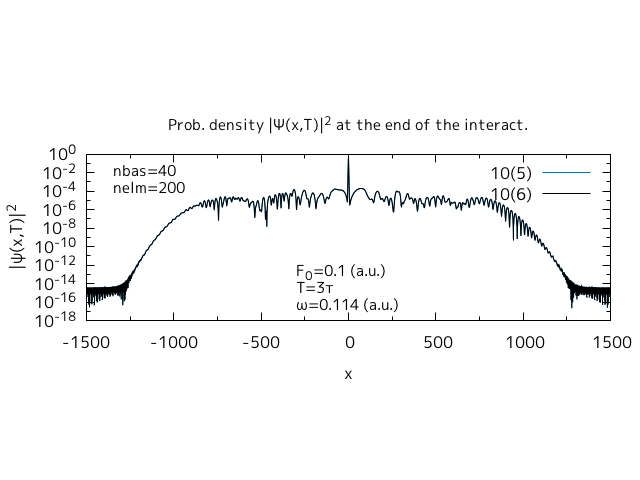
\includegraphics[scale=.20, trim={6 100 10 133},clip]{images/114_f01_3_density_comp.png} \\
% 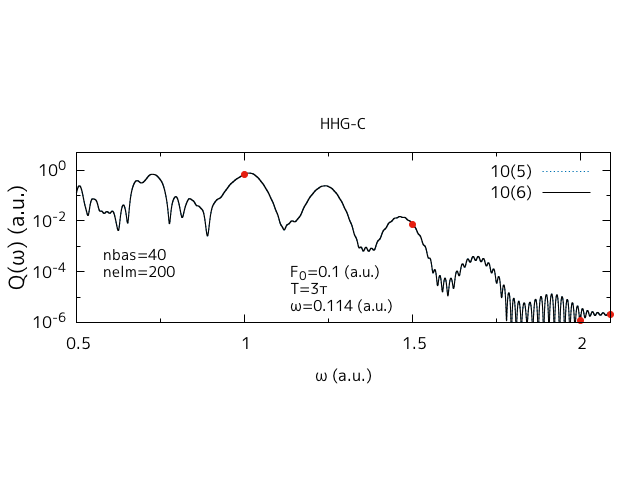
\includegraphics[scale=.20, trim={6 100 10 130},clip]{images/114_f01_3_hhg_comp.png} \\
%% \includegraphics[scale=.20, trim={6 130 10 130},clip]{images/114_f003_8_03_hhg.png} 
%%%\caption{Eigenvalues.}
%%\label{fig:pemd_0114}
% \end{figure}
%
%\end{minipage}
%\end{textblock*}
%
%
%\begin{textblock*}{500pt}(130pt,60pt)
%%\centering
%%\rotatebox{90}{
% \begin{minipage}{0.0\linewidth}
% \begin{figure}[tp]
% 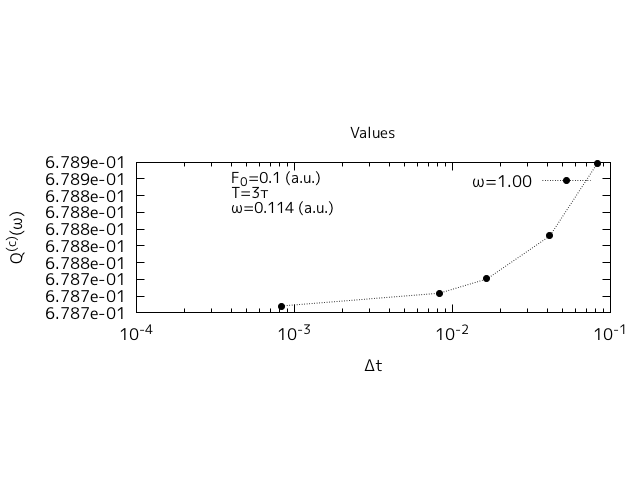
\includegraphics[scale=.20, trim={6 100 10 133},clip]{images/114_f01_3_values_100.png} \\
% 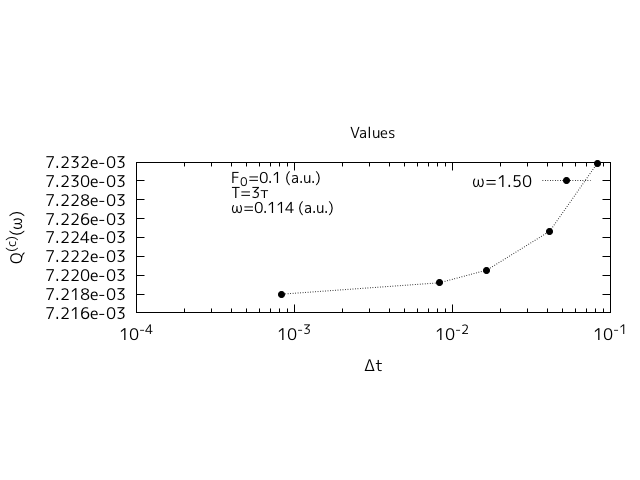
\includegraphics[scale=.20, trim={6 100 10 130},clip]{images/114_f01_3_values_150.png} \\
%% 
\includegraphics[scale=.20, trim={30 130 10 130},clip]{images/114_f003_12_07_hhg.png} 
%%%\caption{Eigenvalues.}
%%\label{fig:pemd_0114}
% \end{figure}
%
%\end{minipage}
%\end{textblock*}
%
%
%\begin{textblock*}{500pt}(255pt,60pt)
%%\centering
%%\rotatebox{90}{
% \begin{minipage}{0.0\linewidth}
% \begin{figure}[tp]
% 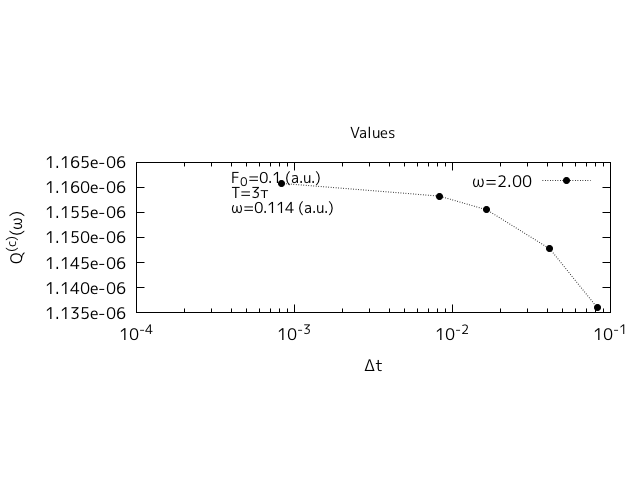
\includegraphics[scale=.20, trim={6 100 10 133},clip]{images/114_f01_3_values_200.png} \\
% 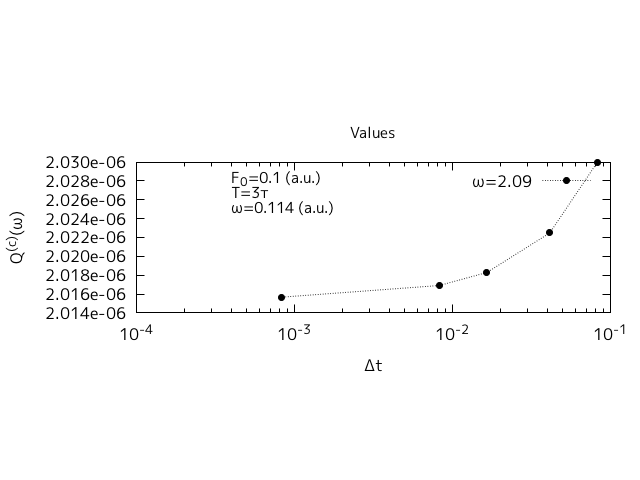
\includegraphics[scale=.20, trim={6 100 10 130},clip]{images/114_f01_3_values_209.png} \\
%% 
\includegraphics[scale=.20, trim={30 130 10 130},clip]{images/114_f003_12_07_hhg.png} 
%%%\caption{Eigenvalues.}
%%\label{fig:pemd_0114}
% \end{figure}
%
%\end{minipage}
%\end{textblock*}
%
%
%\begin{textblock*}{500pt}(390pt,165pt)
%%\centering
%\rotatebox{90}{
% \begin{minipage}{0.0\linewidth}
% \begin{figure}[tp]
% 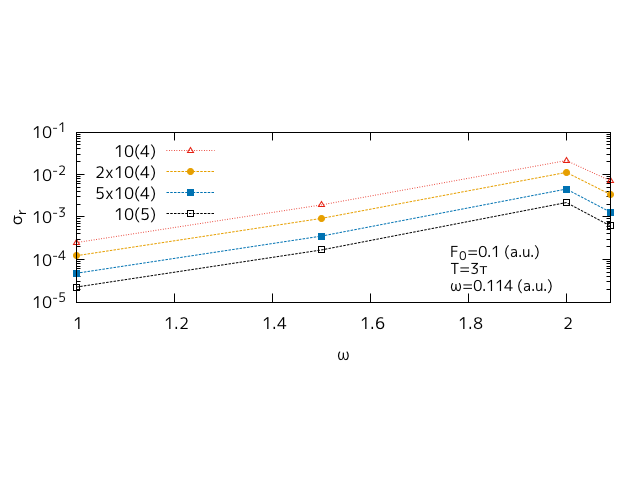
\includegraphics[scale=.20, trim={6 100 10 120},clip]{images/114_f01_3_error.png } \\
%%%\caption{Eigenvalues.}
%%\label{fig:pemd_0114}
% \end{figure}
%\end{minipage}
%}
%}
%\end{textblock*}
%
%
%
%
%\begin{textblock*}{\linewidth}(20pt,170pt)
%\rotatebox{0}{
%\begin{minipage}{\linewidth}
%{
%\tiny 
%\centering
%\input{tables/114_f01_3t_error_2.tab}
%}
%\end{minipage}
%}
%\end{textblock*}
%
%
%\begin{textblock*}{400pt}(30pt,205pt)
%\scriptsize
%
%\begin{align}
%    \sigma_{ij}= \left|\frac{\left(   Q^{(c)}(\omega)[i] 
%       - Q^{(c)}(\omega)[j]  \right)}{Q^{(c)}(\omega)[j]}\right|, \hspace{20pt}
%    Q^{(c)}(\omega) & = \left|\Bigg[ e^{i\omega t} x(t)\Bigg]_{-T/2}^{T/2}
%               -i\omega \int_{-T/2}^{T/2} e^{i\omega t}x(t)dt\right|^2.
%                \nonumber
%\end{align}
%
%\end{textblock*}
%
%\end{frame}


